\newpage
\section{Kenngrössen Turbinen}

\subsection{Hydraulische Leistung}

$\boxed{P_{\text{hyd}} = \rho \cdot Q \cdot g \cdot H_n}$

\vspace{0.15cm}

\renewcommand{\arraystretch}{1.2} % Erhöht Zeilenhöhe für bessere Lesbarkeit
\begin{tabular}{@{} l p {7cm} l @{}}
    $[P_{\text{hyd}}]$  & Hydraulische Leistung \dotfill & $\mathrm{W}$ \\
    $[Q]$               & Nutzwassermenge \dotfill & $\mathrm{\frac{m^3}{s}}$ \\
    $[H_n]$             & Nettofallhöhe \dotfill & $\mathrm{m}$ \\
    $[\rho]$            & Dichte des Wassers ($\rho = 1000$) \dotfill & $\mathrm{\frac{kg}{m^3}}$ \\
    $[g]$               & Erdbeschleunigung ($g = 9.81$) \dotfill & $\mathrm{\frac{m}{s^2}}$ \\
\end{tabular}



\subsection{Mechanische Leistung an der Turbinenwelle}

$\boxed{P_{\text{mech}} = \omega \cdot M} \quad \boxed{P_{\text{mech}} = \eta_t \cdot P_{\text{hyd}}}$

\vspace{0.15cm}

\renewcommand{\arraystretch}{1.2} % Erhöht Zeilenhöhe für bessere Lesbarkeit
\begin{tabular}{@{} l p {6cm} l @{}}
    $[P_{\text{mech}}]$  & Mechanische Leistung   \dotfill & $\mathrm{W}$ \\
    $[\omega]$           & Winkelgeschwindigkeit \dotfill & $\mathrm{\frac{rad}{s}}$ \\
    $[\eta_t]$           & Wirkungsgrad Turbine \dotfill & $-$ \\
    $[M]$                & Drehmoment            \dotfill & $\mathrm{Nm}$ \\
\end{tabular}



\subsection{Winkelgeschwindigkeit}

$\boxed{\omega = 2 \cdot \pi \cdot n}$

\vspace{0.15cm}

\renewcommand{\arraystretch}{1.2} % Erhöht Zeilenhöhe für bessere Lesbarkeit
\begin{tabular}{@{} l p {6cm} l @{}}
    $[\omega]$  & Winkelgeschwindigkeit \dotfill & $\mathrm{\frac{rad}{s}}$ \\
    $[n]$       & Drehzahl              \dotfill & $\mathrm{\frac{1}{s}}$ \\
\end{tabular}



\subsection{Betriebszustände der Maschinengruppe}
\textbf{(Maschinengruppe = Turbine/Pumpe + Generator/Motor)}

\begin{itemize}
    \item Inselbetrieb
    \item Parallelbetrieb, Verbundbetrieb
    \item Instationäre Vorgänge
    \begin{itemize}
        \item Anfahren und Abstellen
        \item Lastabwurf $\Rightarrow$ Überdrehzahl
    \end{itemize}
\end{itemize}

\textbf{Durchgangsdrehzahl $n_D$} (auch Schleuderdrehzahl genannt)

$\Rightarrow$ höchste erreichbare Drehzahl ohne Last (z.B. bei Versagen des Generators)

Die Durchgangsdrehzahl ist eine Bemessungsgröße. 

Die Maschinengruppe darf bei der Durchgangsdrehzahl keinen Schaden erleiden.

\subsection{Spezifische Drehzahl $n_q$}

\noindent
$
\boxed{
n_q = n \cdot \frac{\sqrt{Q}}{H_n^{3/4}}
}
$

\vspace{0.15cm}

\renewcommand{\arraystretch}{1.2}
\begin{tabular}{@{} l p{6cm} l @{}}
    $[n_q]$          & Spezifische Drehzahl \dotfill                               & $\text{U/min}$ \\
    $[n]$            & Drehzahl der Turbine \dotfill                               & $\text{U/min}$ \\
    $[Q]$            & Nutzwassermenge \dotfill                                    & $\frac{\text{m}^3}{\text{s}}$ \\
    $[H_n]$          & Nettofallhöhe \dotfill                                      & $\text{m}$ \\
\end{tabular}

\vspace{0.15cm}

$n_q$ ist die Drehzahl einer Turbine in \(\mathrm{U/min}\), welche bei einem Gefälle von \(1 \,\mathrm{m}\) einen Volumenstrom von \(1 \,\mathrm{m}^3/\mathrm{s}\) aufweist (Ähnlichkeitsgesetz).




\myul{\textbf{Typische $n_q$}}

\vspace{0.15cm}

\textbf{Peltonturbinen} \hspace{1cm} $<$ 20 U/min 

\vspace{0.15cm}

\textbf{Francisturbinen} \hspace{1cm} ca. 20 bis ca. 100 U/min 

\vspace{0.15cm}

\textbf{Kaplanturbinen} \hspace{1cm} $>$ 100 U/min



\newcolumn
\section{Turbinen}

\subsection{Peltonturbine}

\begin{minipage}[c]{0.48\columnwidth}
    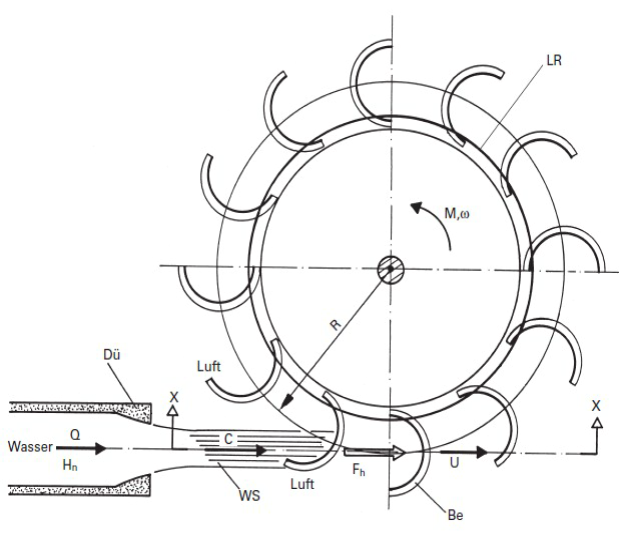
\includegraphics[width=0.98\columnwidth, align=c]{images/Pelton_Turbine_1.png}    
\end{minipage}
\hfill
\begin{minipage}[c]{0.48\columnwidth}
    \includegraphics[width=0.98\columnwidth, align=c]{images/Pelton_Turbine_2.png}   
\end{minipage}

\begin{tabular}{c l}
    a & Peltonrad \\
    b & Düse \\
    c & Strahlablenker \\
    d & Bremsdüse \\
\end{tabular}

\vspace{0.15cm}

\begin{minipage}[c]{0.48\columnwidth}
    Düse offen    
\end{minipage}
\hfill
\begin{minipage}[c]{0.48\columnwidth}
    Düse geschlossen   
\end{minipage}

\begin{minipage}[c]{0.48\columnwidth}
    \includegraphics[width=0.98\columnwidth, align=c]{images/Pelton_Turbine_Düse_offen.png}    
\end{minipage}
\hfill
\begin{minipage}[c]{0.48\columnwidth}
    \includegraphics[width=0.98\columnwidth, align=c]{images/Pelton_Turbine_Düse_geschlossen.png}   
\end{minipage}

\begin{tabular}{c l}
        1 & Düsennadel \\
        2 & Kolben \\
        3 & Öl zum öffnen \\
        4 & Öl zum Schliessen \\
        5 & Rückmeldung
\end{tabular}

\subsubsection{Eingenschaften und Merkmale}
\begin{itemize}
    \item Guter Wirkungsgrad über einen großen Einsatzbereich von 10 bis 100\% der max. Leistung
    \item Unkritische Maschine
    \item Der sogenannte Gletscherschliff muss beachtet werden (Erosion am Laufrad)
    \item Verschraubung Rad- / Generatorflansch (Kupplung) mit z.B. mechanisch vorgespannten Dehnschrauben
    \item Trockenenlegung der Kupplung
    \item Wirkungsgradverbesserungen oft möglich
    \item Rissen im Bereich der Becherwurzel (hochbelastete Zone) gilt ein spezielles Augenmerk
\end{itemize}



\subsection{Reaktionsturbinen}

\begin{itemize}
    \item Francisturbinen
    \item Kaplanturbinen
    \item Rohrturbinen
    \item Kreiselpumpen als Turbinen
\end{itemize}



\subsubsection{Funktionsprinzip}

\textbf{Turbinenspirale (TS)}: exzentrisch zur Turbinenachse angeordneter Zulaufkanal, der die durch eine \textbf{Turbinenspirale} erzeugte Drallströmung (\textbf{DS}) veranschaulicht (<<Badewannenablass>>)

\textbf{Laufrad (LR)}: Schaufelrad, welches das in der \textbf{Drallströmung} DS platzierte Laufrad der Turbine darstellt

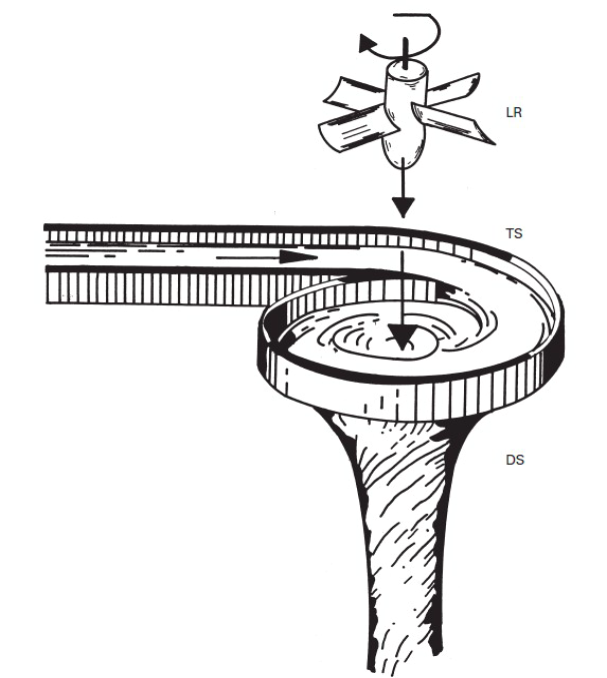
\includegraphics[width=0.58\columnwidth, align=c]{images/Laufradturbinen.png}   



\subsubsection{Kavitation}

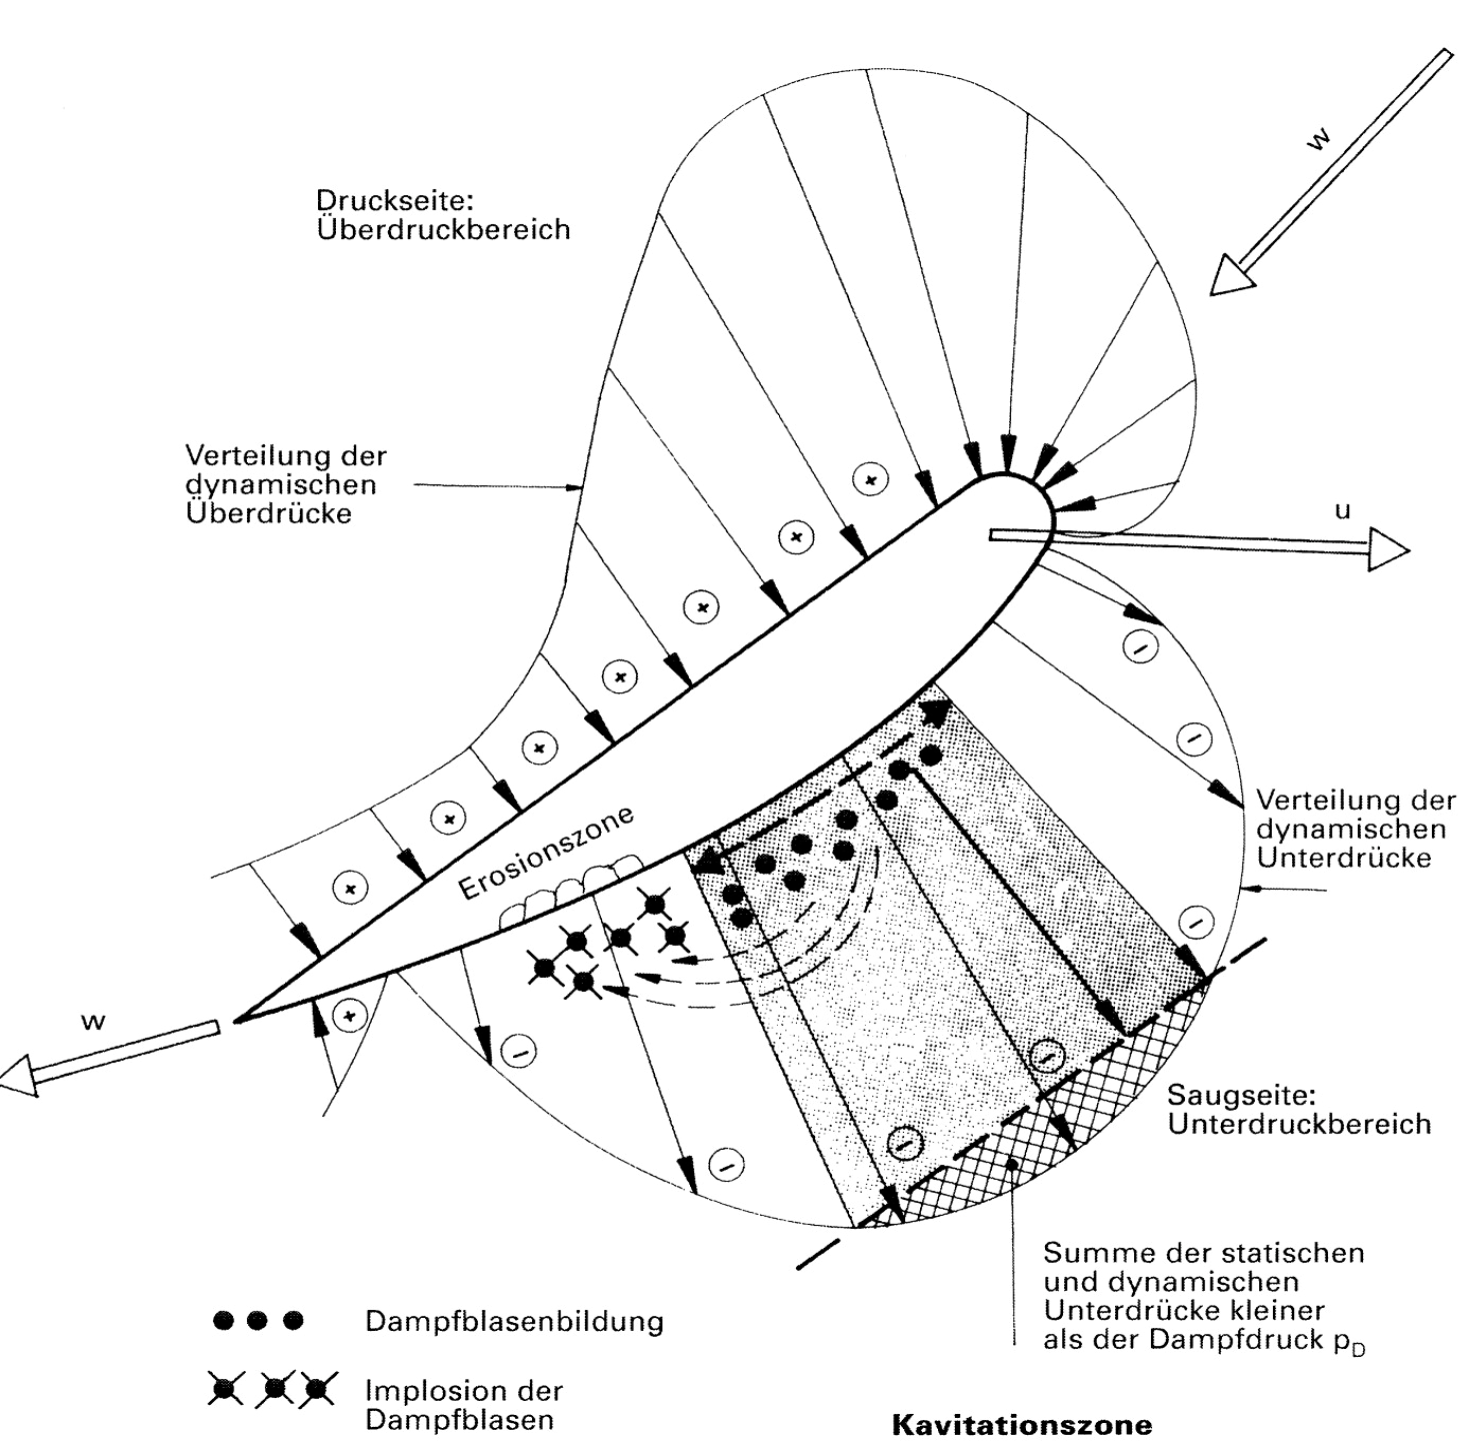
\includegraphics[width=0.98\columnwidth, align=c]{images/Kavitation.png}   

\renewcommand{\arraystretch}{1.2} % Erhöht Zeilenhöhe für bessere Lesbarkeit
\begin{tabular}{@{} l p {7cm} l @{}}
    $[w]$   & Rel. Geschw. des Wassers bez. der drehenden Schaufel  \dotfill & $\mathrm{\frac{m}{s}}$ \\
    $[u]$   & Umfanggeschwindigkeit der Schaufel                    \dotfill & $\mathrm{\frac{m}{s}}$ \\
\end{tabular}

\vspace{0.15cm}

\begin{tabular}{ll}
\hline
\textbf{Turbinentyp} & \({n_D}/{n_N}\) \\
\hline
Francis, \(n_q = 40 \ldots 80\) U/min & \(1.7 \ldots 2.0\) \\
Francis, \(n_q = 80 \ldots 120\) U/min & \(2.0 \ldots 2.2\) \\
Propeller, feste Lauf- und Leitschaufeln & \(1.8 \ldots 2.2\) \\
Kaplan, verstellbare Laufschaufeln, feste Leitschaufeln & \(2.4 \ldots 2.8\) \\
Kaplan, verstellbare Lauf- und Leitschaufeln & \(2.4 \ldots 3.2\) \\
Pumpen im Turbinenbetrieb, \(n_q = 30 \ldots 100\) U/min & \(1.4 \ldots 1.8\) \\
\hline
\end{tabular}

\vspace{0.15cm}

Je grösser \({n_D}/{n_N}\) desto stärker muss die Turbine dimensioniert werden

\vspace{0.15cm}

\textbf{Verhältnis der Volumenströme bei Durchgangs- bzw. Nenndrehzahl:}

$
\begin{aligned}
   n_q < 100 \ \mathrm{U/min:} & \quad Q_D < Q_N \\
    n_q = 100 \ \mathrm{U/min:} & \quad Q_D = Q_N \\
    n_q > 100 \ \mathrm{U/min:} & \quad Q_D > Q_N 
\end{aligned}
$

\vspace{0.15cm}

\begin{itemize}
    \item \textbf{Durchgangsdrehzahl} \(n_D\)
    \item \textbf{Nenndrehzahl} \(n_N\)
    \item \textbf{Spezifische Drehzahl} \(n_q\)
\end{itemize}

\vspace{0.15cm}

\renewcommand{\arraystretch}{1.2} % Erhöht Zeilenhöhe für bessere Lesbarkeit
\begin{tabular}{@{} l p {7cm} l @{}}
    $[n_D]$   & Drehzahl bei Lastabwurf (plötzlicher Generatorverlust)  \dotfill & $\mathrm{\frac{U}{min}}$ \\
    $[n_N]$   & Tatsächliche Drehzahl im Normalbetrieb                    \dotfill & $\mathrm{\frac{U}{min}}$ \\
    $[n_q]$   & Drehzahl einer skalierten Maschine  \(\left(H = 1\,\mathrm{m},\, Q = 1\,\mathrm{m}^3/\mathrm{s}\right)\)                  \dotfill & $\mathrm{\frac{U}{min}}$ \\
\end{tabular}



\subsection{Francisturbinen}

\begin{minipage}[c]{0.48\columnwidth}
    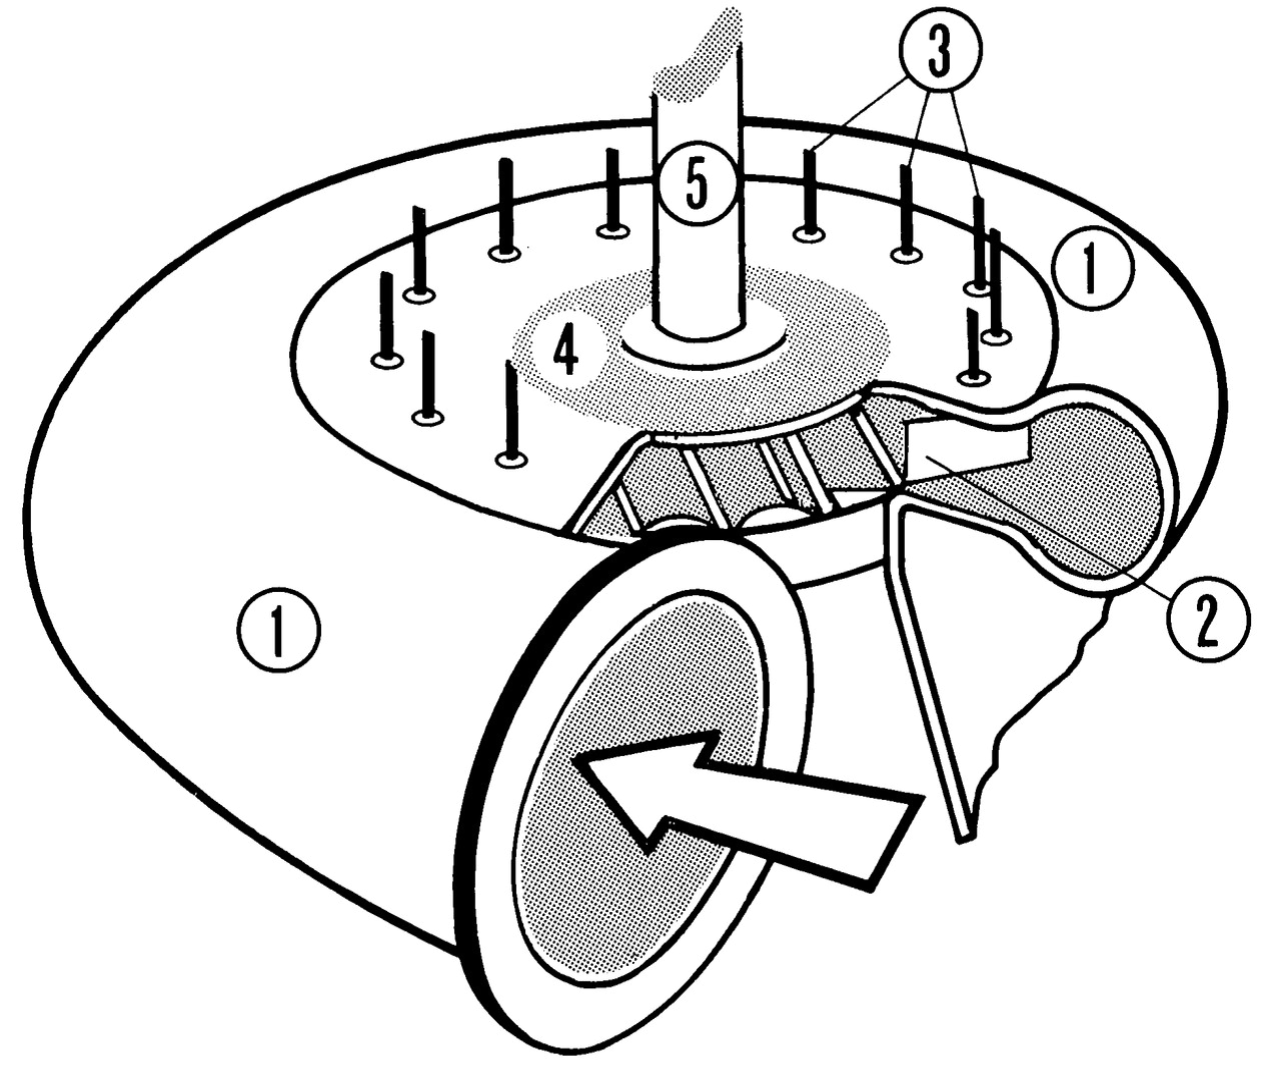
\includegraphics[width=0.98\columnwidth, align=c]{images/Francis_Turbine.png}    
\end{minipage}
\hfill
\begin{minipage}[t]{0.48\columnwidth}
    \begin{tabular}{c l}
        1 & Einlaufspirale \\
        2 & Leitschaufeln \\
        3 & Leitschaufelnachse \\
        4 & Laufrad \\
        5 & Turbinenwelle
\end{tabular}  
\end{minipage}



\subsection{Kaplanturbinen}

\begin{minipage}[c]{0.48\columnwidth}
    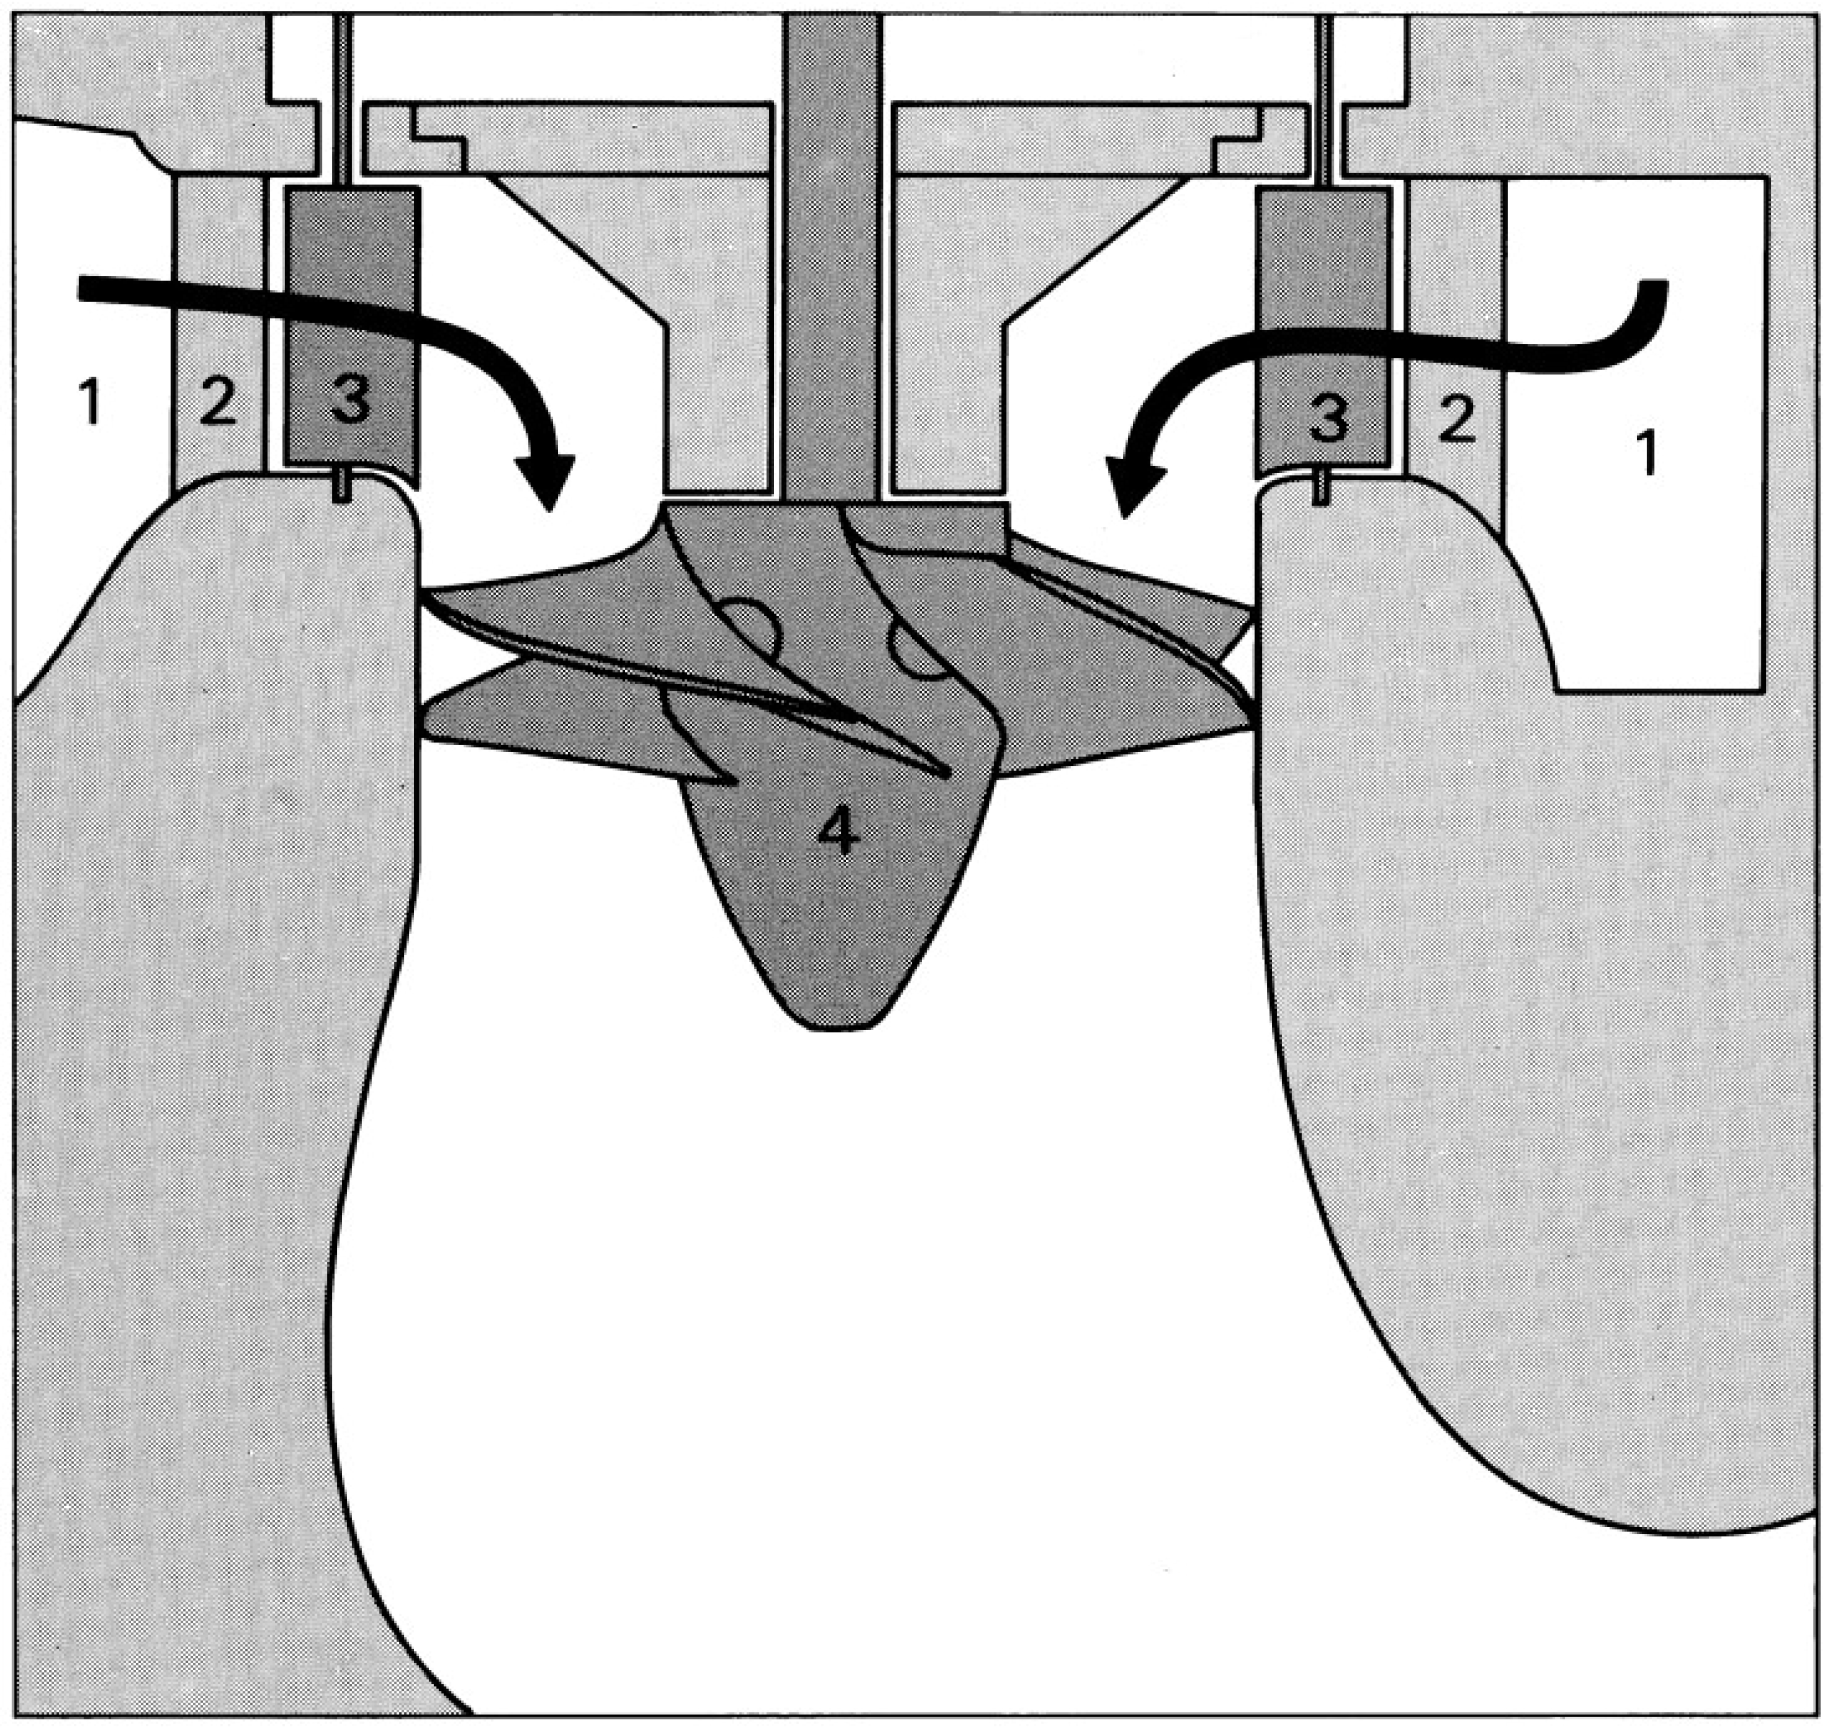
\includegraphics[width=0.98\columnwidth, align=c]{images/Kaplan_Turbine.png}    
\end{minipage}
\hfill
\begin{minipage}[t]{0.48\columnwidth}
    \begin{tabular}{c l}
        1 & Einlaufspirale \\
        2 & Stützschaufeln \\
        3 & Leitschaufeln \\
        4 & Kaplan-Rad \\
\end{tabular}  
\end{minipage}



\subsection{Rohrturbinen (= horizontale Kaplanturbinen)}

\begin{minipage}[c]{0.48\columnwidth}
    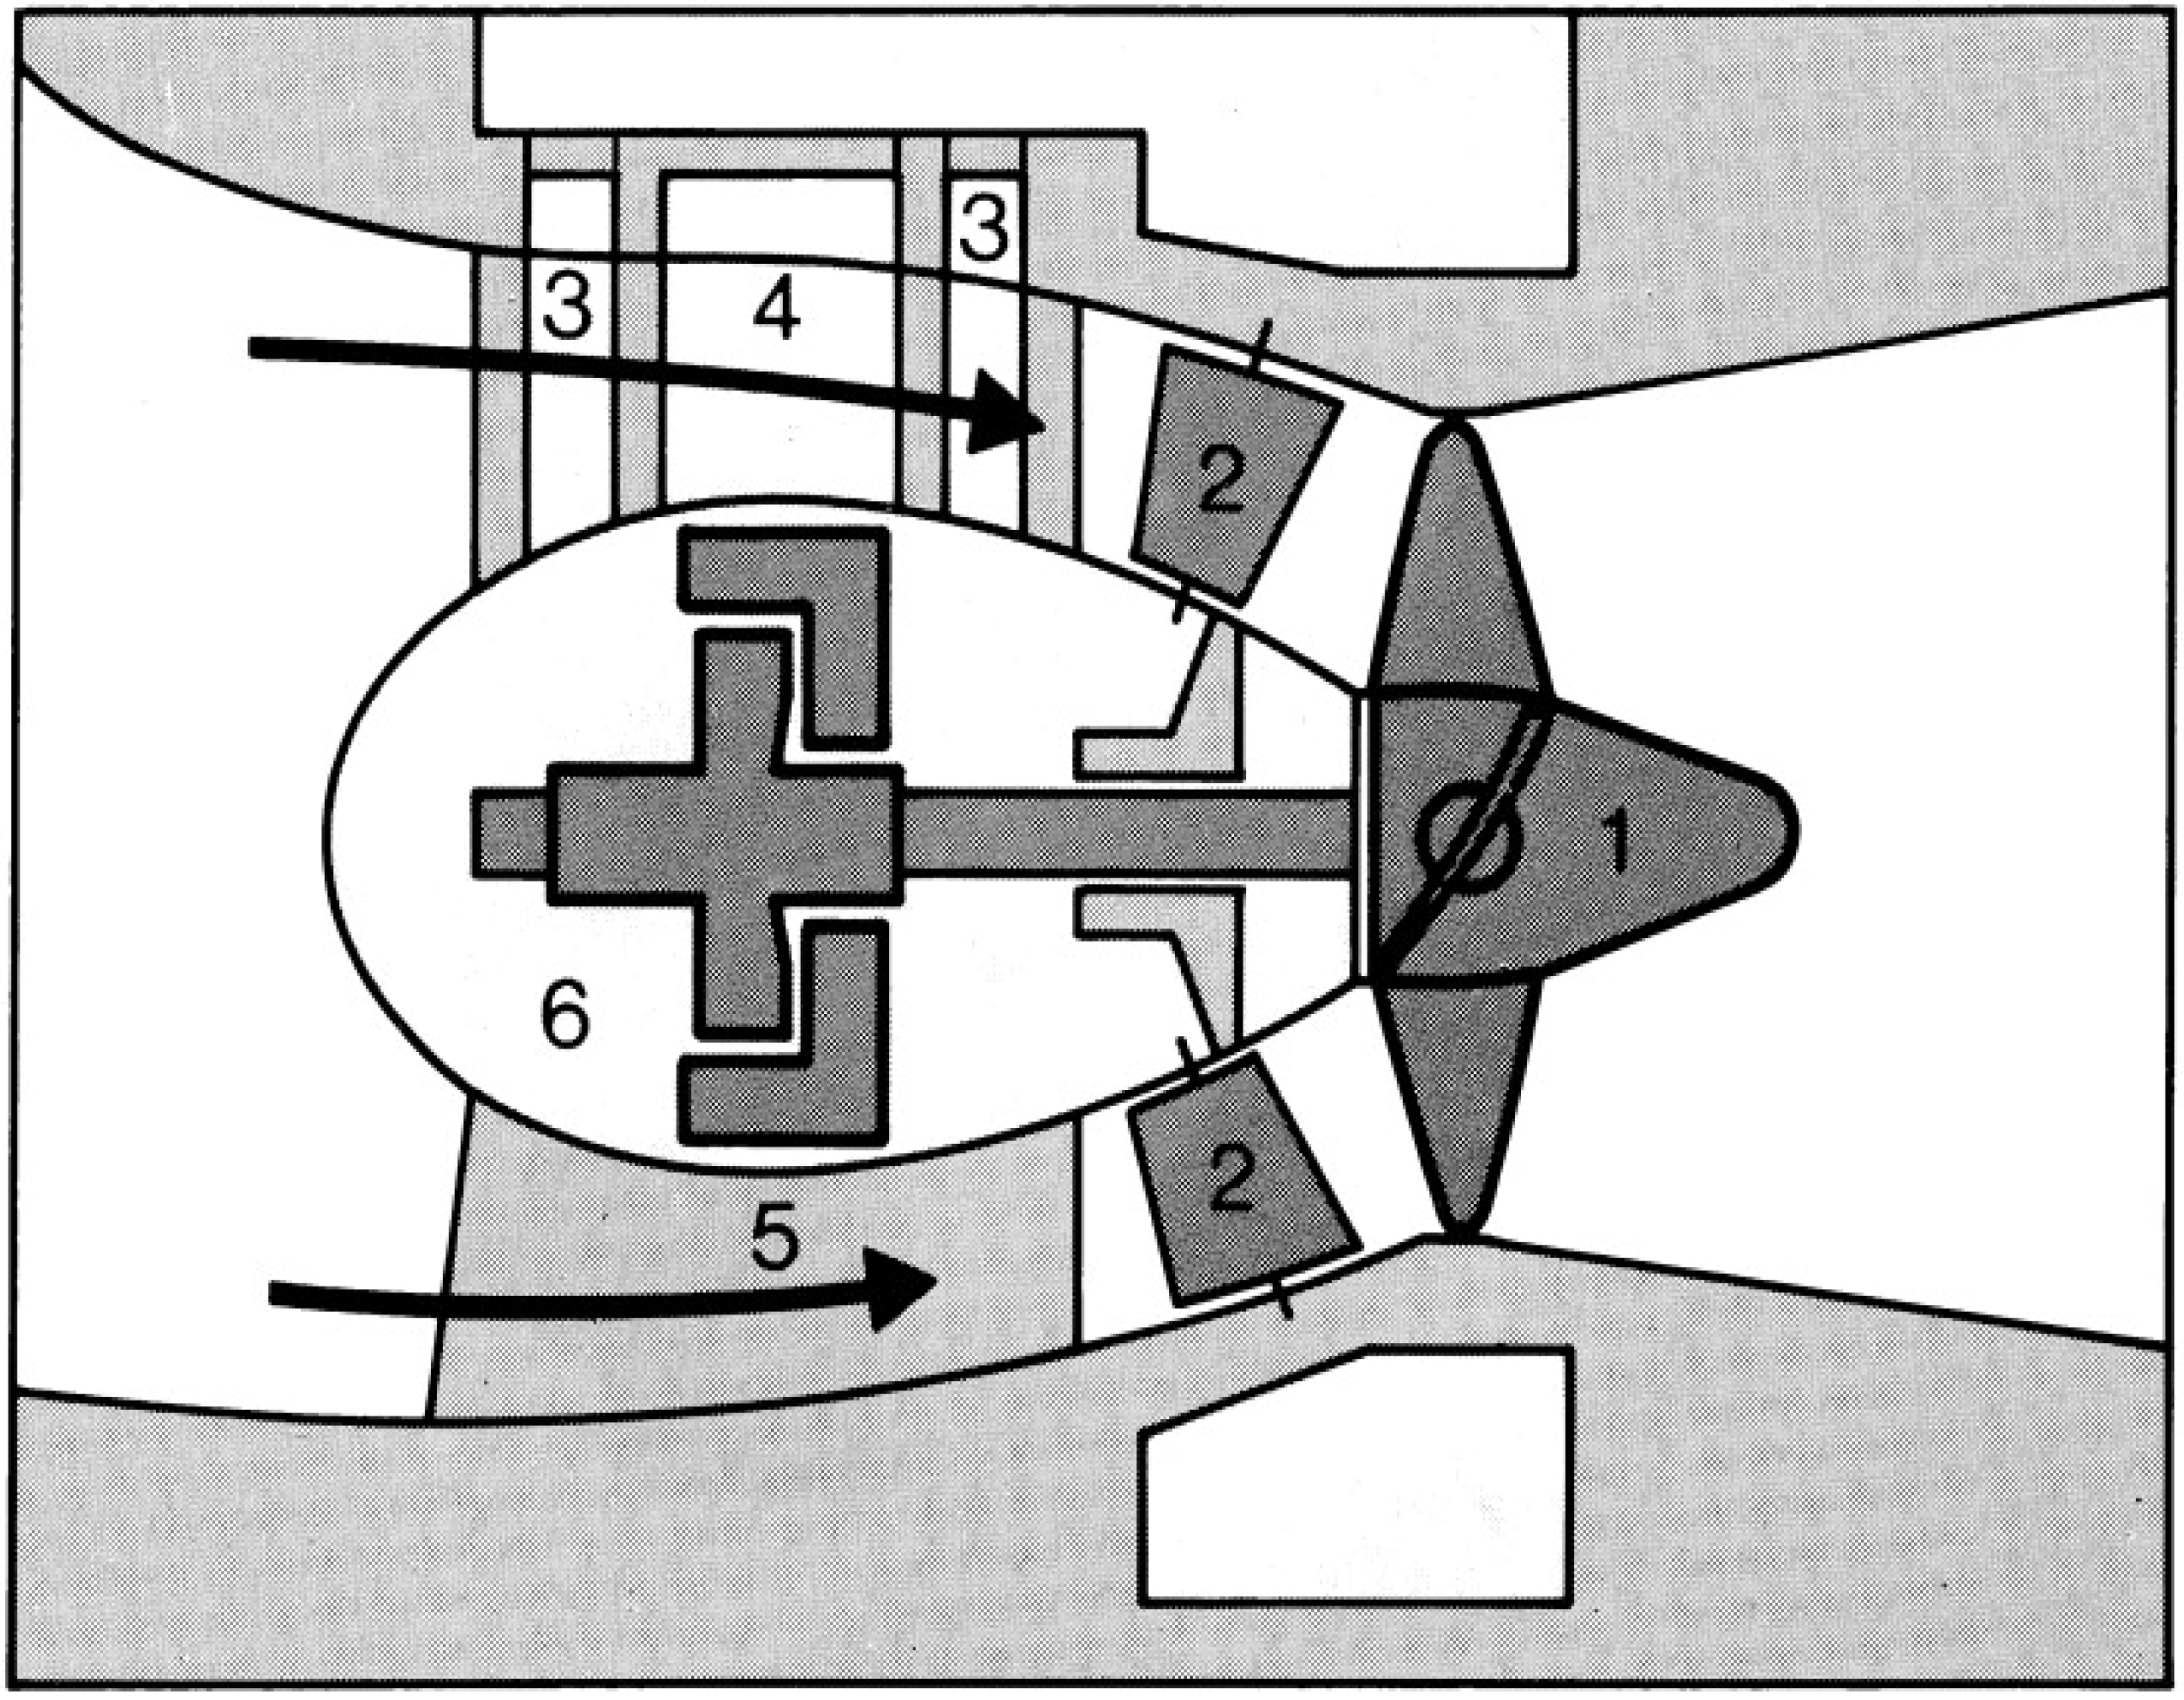
\includegraphics[width=0.98\columnwidth, align=c]{images/Rohr_Turbinen.png}    
\end{minipage}
\hfill
\begin{minipage}[t]{0.48\columnwidth}
    \begin{tabular}{c l}
        1 & Schaufelrad \\
        2 & Leitschaufeln \\
        3 & Zustiegsschächte \\
        4 & Demontageschacht \\
        5 & Sockel \\
        6 & Generator \\
\end{tabular}  
\end{minipage}



\subsection{Strafloturbinen}
\begin{minipage}[c]{0.48\columnwidth}
    \includegraphics[width=0.98\columnwidth, align=c]{images/Straflo_Turbine.png}    
\end{minipage}
\hfill
\begin{minipage}[t]{0.48\columnwidth}
    \begin{tabular}{c l}
        1 & Laufradschaufeln \\
        2 & Rotor, Pole des Generators \\
        3 & Stator \\
        4 & Leitschaufeln \\
\end{tabular}  
\end{minipage}

\subsection{Speicherpumpen und Pumpturbinen}
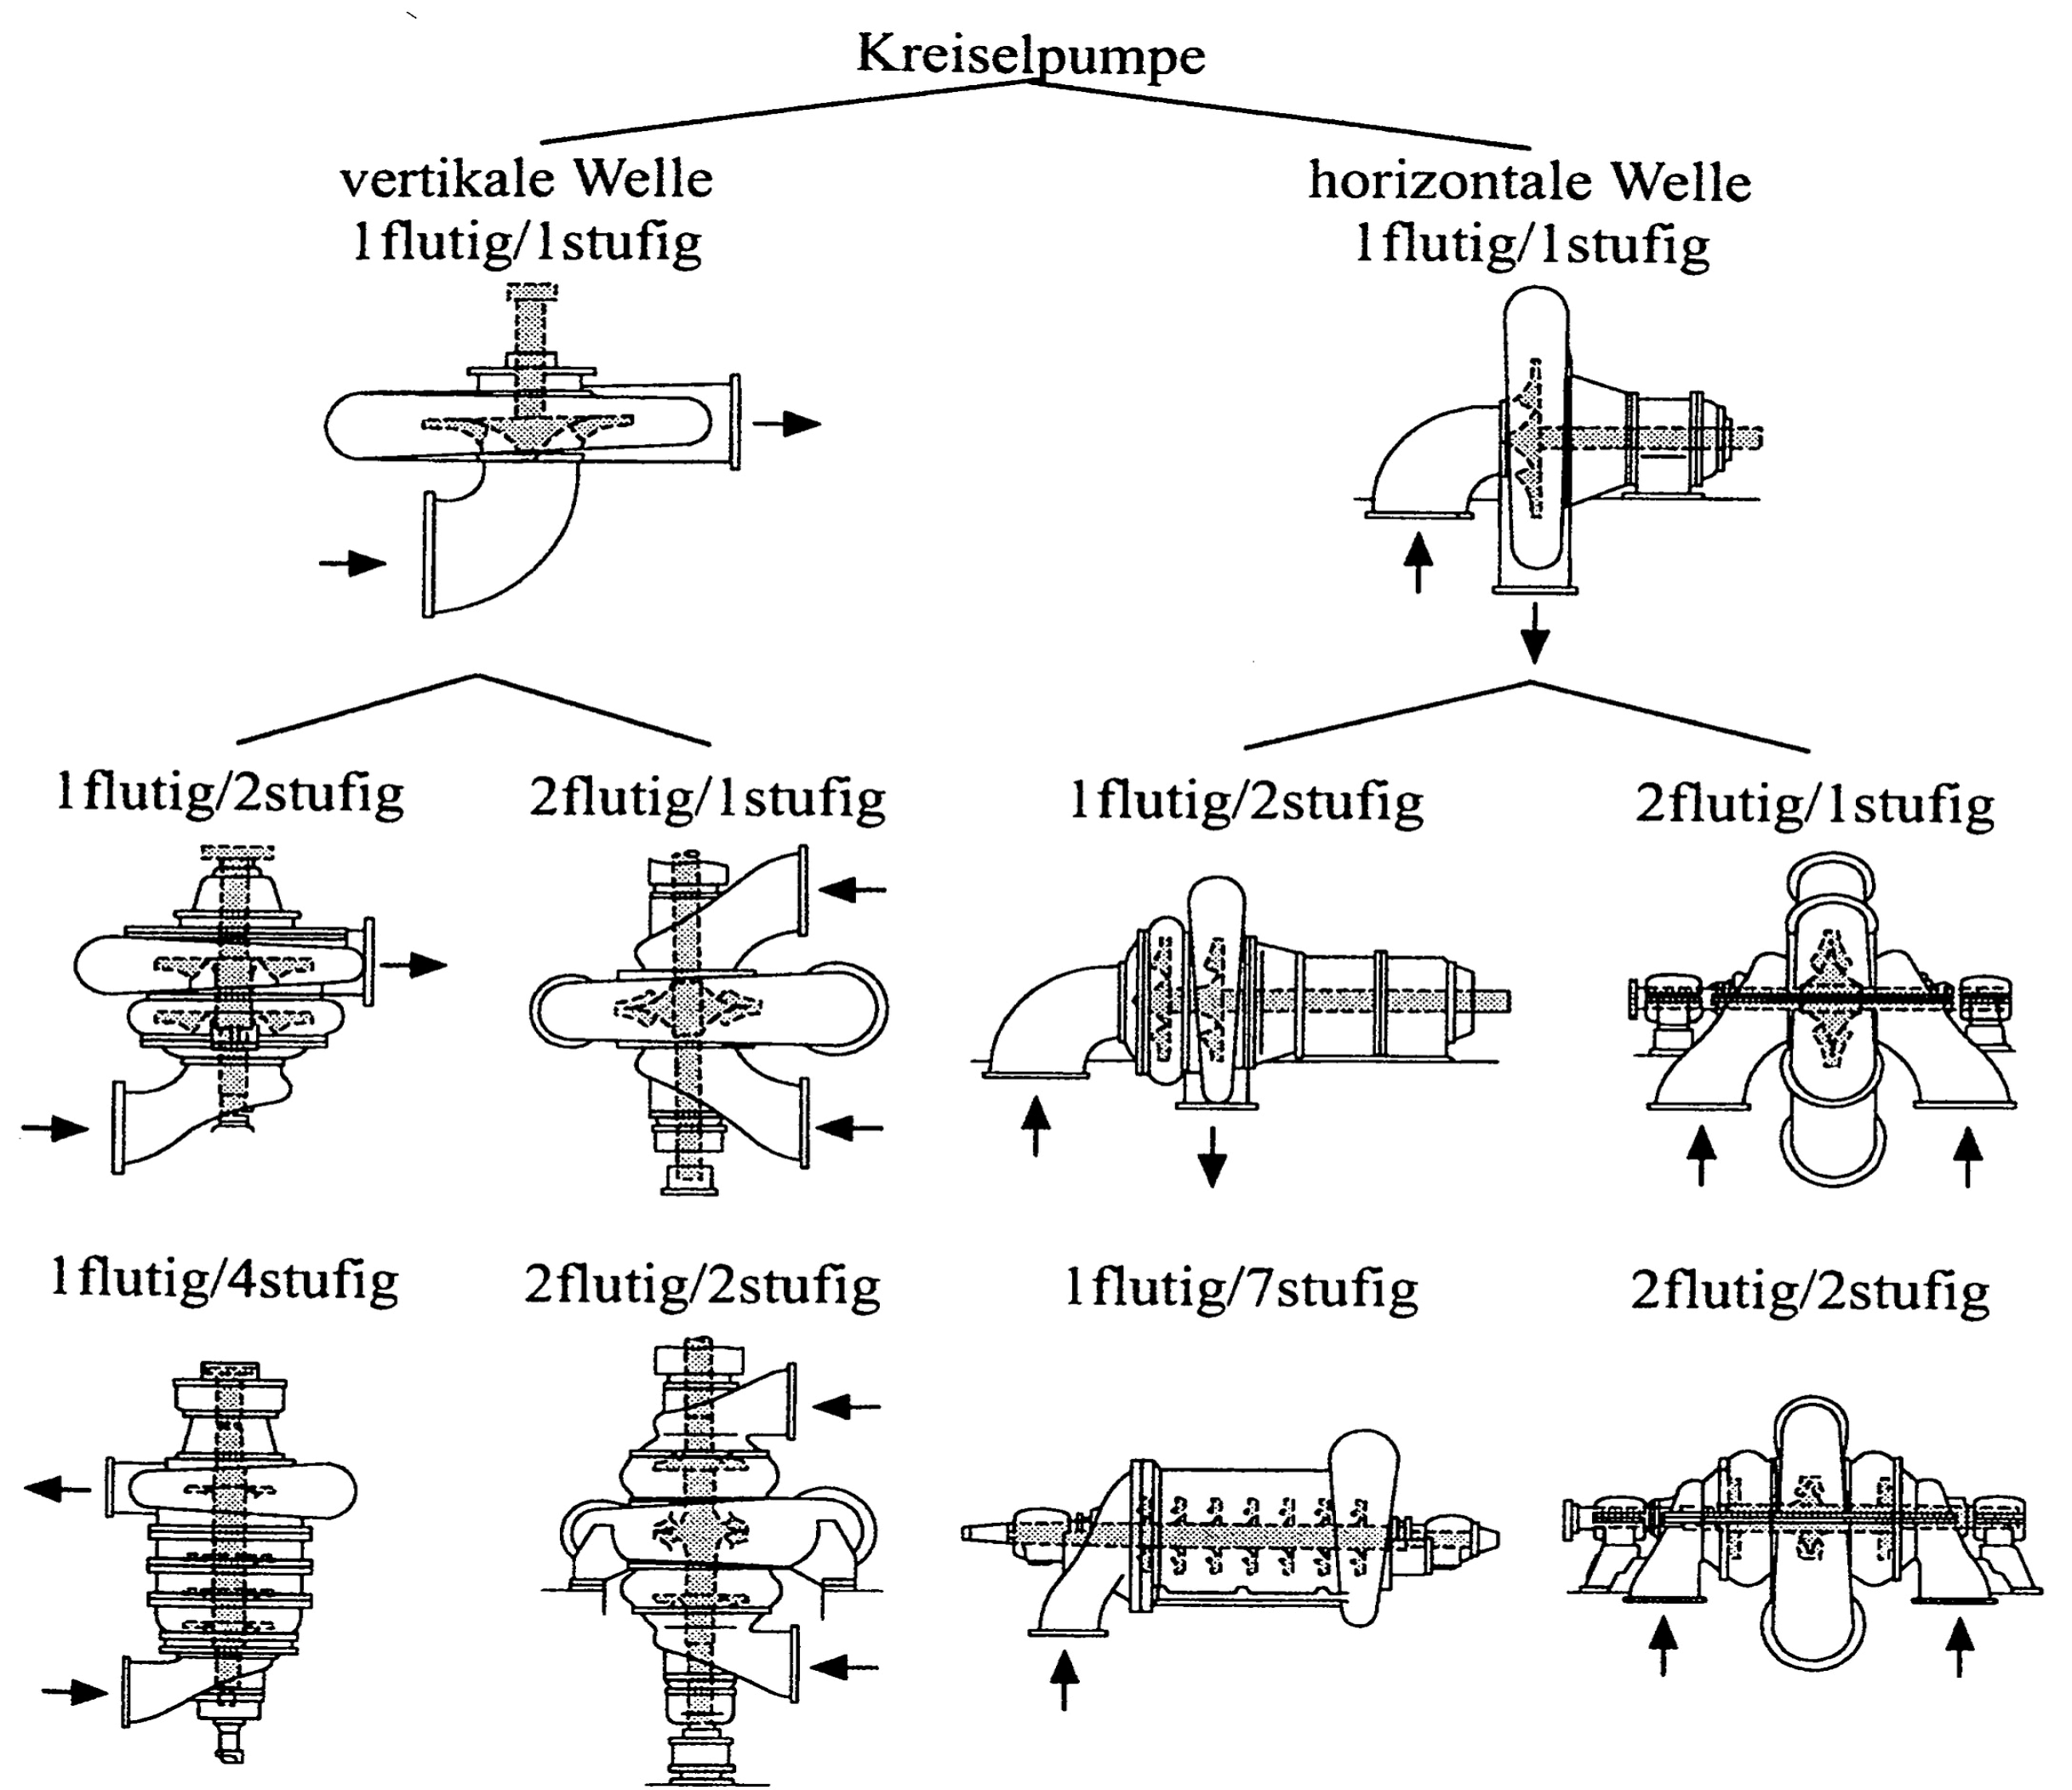
\includegraphics[width=0.98\columnwidth, align=c]{images/Speicherpumpen und Pumpturbinen.png}   

\subsubsection{Dreimaschinensatz}

Besteht aus: Generator/Motor, Francisturbine und Speicherpumpe

\vspace{0.15cm}

    \textcolor{red}{\textbf{Nachteile}} 
    \begin{itemize}
        \item Zwei hydraulische Maschinen sowie eine größere Anzahl Abschlussorgane sind nötig.
    \end{itemize}
    \textcolor{green}{\textbf{Vorteil}}
    \begin{itemize}
        \item Unabhängige Optimierung der Turbine und der Pumpe ist möglich.
    \end{itemize}




\subsection{Wahl des Generators}

Der Generator muss synchron mit dem Netz drehen. Daher muss die definitive Drehzahl der in der Nähe liegenden Synchrondrehzahl entsprechen.

\vspace{0.15cm}

$
\boxed{n = 60 \cdot \frac{f}{p} } \quad \boxed{n = \frac{3000}{p}}
$

\vspace{0.15cm}

\renewcommand{\arraystretch}{1.2}
\begin{tabular}{@{} l p{6cm} l @{}}
    $[n]$           & Drehzahl des Generators \dotfill                         & $\text{U/min}$ \\
    $[f]$           & Frequenz, meist 50 Hz \dotfill                            & $\text{Hz} = \frac{1}{\text{s}}$ \\
    $[p]$           & Polpaarzahl \dotfill                                      & (1, 2, 3, \dots) \\
\end{tabular}


\subsection{Kochrezept zur Grob-Auslegung von Pumpen und Turbinen}

\begin{enumerate}
    \item Bestimmung der \textbf{Netto-Fallhöhe} \( H_n \)
    \item Auswahl \textbf{Gesamtdurchfluss} \( Q \), abhängig von Zufluss, Rückhaltemöglichkeit, Einsatztyp (z.B. Spitzenlast)
    \item Bestimmung der \textbf{hydraulischen Leistung}:
    \[
    P_\mathrm{hyd} = \rho \cdot Q \cdot g \cdot H_n
    \]
    \item Auswahl \textbf{Turbinentyp}, \textbf{Turbinen-Durchfluss} \( Q \) und \textbf{spezifische Drehzahl} \( n_q \) aus Diagrammen\\
    (ggf. Aufteilung \( Q \) auf mehrere Turbinen / Pumpen)
    \item Bestimmung der \textbf{Turbinen-Drehzahl}:
    \[
    n = n_q \cdot \frac{H_n^{3/4}}{Q^{1/2}}
    \]
    \item Bestimmung der \textbf{Polpaarzahl}:
    \[
    p = \frac{3000}{n}
    \]
    (auf ganze Zahl runden und prüfen, ob \( n_q \) nach Rundung noch im möglichen Bereich liegt)
    \item Weitere Bedingungen zur \textbf{Feinauslegung}:
    \begin{itemize}
        \item Teillastverhalten, Wirkungsgrad, Betriebsbereiche
        \item Räumliche Bedingungen, Simulationen, Experimente
        \item \(\ldots\)
        \item Lösung ist ein Abwägen und iterativer Prozess
    \end{itemize}
\end{enumerate}


















